\documentclass[12pt]{article}

\title{A visual method for generating the separating isosurface of two classes of objects in two-dimensional space}
\author{
Shawn Halayka\footnote{Independent -- sjhalayka@gmail.com}
}


\date{\today\;\currenttime}

\usepackage{datetime}
\usepackage{listings}
\usepackage{cite}
\usepackage{xcolor}
\usepackage{graphicx}
\usepackage{setspace}
\usepackage{amsmath}
\usepackage{url}
\usepackage{amsfonts}
\usepackage{caption}
\usepackage{subcaption}

\usepackage[margin=1in]{geometry}

%\doublespace

\begin{document}




\maketitle

\begin{abstract}
With regard to the separating isosurface of two classes of objects in two-dimensional space, the transition from curvilinear to rectilinear is documented.
OpenCV and Marching Squares were used to calculate the data that were used for illustrations in this paper.
\end{abstract}




\section{Introduction}

In terms of statistical learning, a balance between high variance (curvilinearity) and high bias (rectilinearity) is to be had \cite{james}.

Marching Squares works as a radial (spherical) isosurface generator, as well as a rectilinear (planar) isosurface generator -- it all depends on the grid resolution.
The data generated by Marching Squares are the line segments that separate the two classes, as well as triangles for the area of each class.
Classifying a test point is a matter of ray-triangle intersection, which can be accelerated using a Bounding Volume Hierarchy or quadtree data structure.

OpenCV was used to downsize the bitmap image.
OpenCV could also have been used to transform the bitmap image via blur, sharpen, or whatnot -- this visual method practically begs for such experimentation.



\begin{thebibliography}{9}

\bibitem{james} James, et al. An Introduction to Statistical Learning with Applications in R. ISBN: 978-1-0716-1417-4

\end{thebibliography}










\begin{figure} 
\centering
  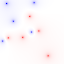
\includegraphics[width = 3 in]{64_res_image.png}
  \caption{Bitmap image used as input to the Marching Squares algorithm. 
Image size is 64x64.
Colour falls off with distance.
}
\end{figure}

\begin{figure} 
\centering
  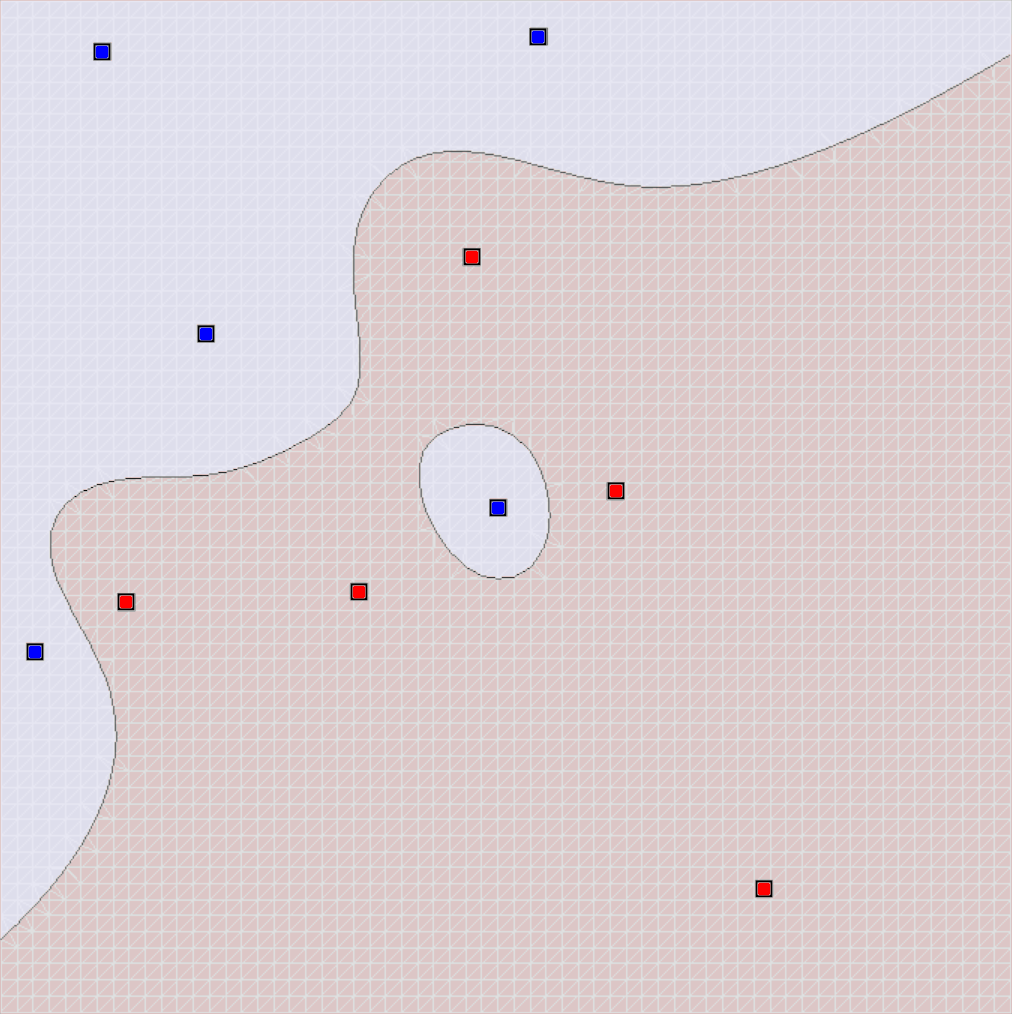
\includegraphics[width = 3 in]{64_res.png}
  \caption{The output of the Marching Squares algorithm: curvilinear, radial separation. Grid resolution is 64x64.
}
\end{figure}


\begin{figure} 
\centering
  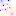
\includegraphics[width = 3 in]{16_res_image.png}
  \caption{Bitmap image used as input to the Marching Squares algorithm.
Image size is 16x16.
}
\end{figure}


\begin{figure} 
\centering
  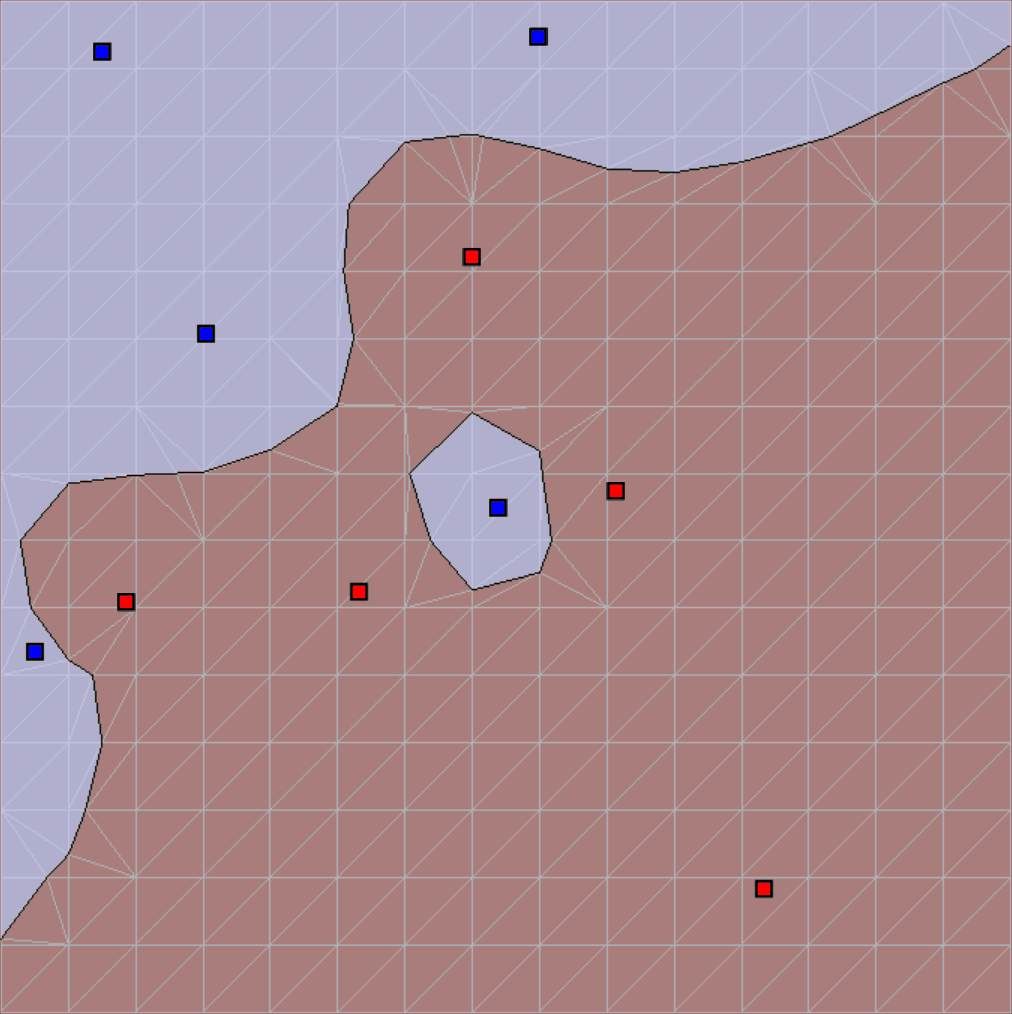
\includegraphics[width = 3 in]{16_res.png}
  \caption{The output of the Marching Squares algorithm: curvilinear, radial separation. Grid resolution is 16x16.
}
\end{figure}

\begin{figure} 
\centering
  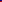
\includegraphics[width = 3 in]{2_res_image.png}
  \caption{Bitmap image used as input to the Marching Squares algorithm.
Image size is 2x2.
}
\end{figure}


\begin{figure} 
\centering
  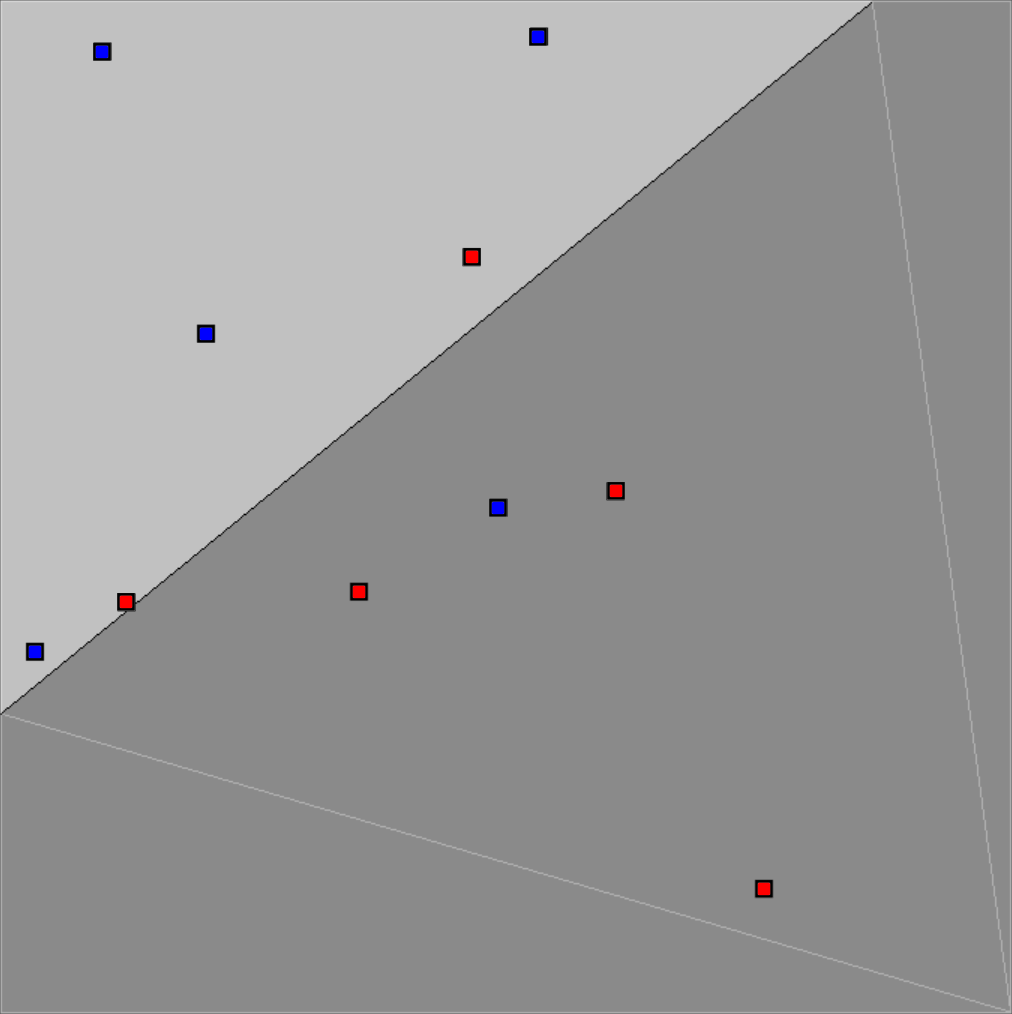
\includegraphics[width = 3 in]{2_res.png}
  \caption{The output of the Marching Squares algorithm: rectilinear separation. Grid resolution is 2x2.
}
\end{figure}












\end{document}









